% !TeX program = xelatex
\documentclass[a4paper,12pt]{extarticle} 
\usepackage{extsizes}
\usepackage{amsmath}
\usepackage{indentfirst}%для абзацев с красной строки
\parindent=1cm
\usepackage[T2A]{fontenc}
\usepackage{setspace}
\usepackage{caption} 
%\captionsetup[figure]{name=Рисунок}
\usepackage[russian]{babel}
\usepackage[utf8]{inputenc}
\usepackage{cmap}
\linespread{1.5} % полуторный интервал
\usepackage{graphicx}
\graphicspath{{images/}}
\usepackage{lscape} 
\usepackage{longtable}
\usepackage{geometry}
\usepackage{breqn}
\usepackage{color}
\usepackage{hyperref}
%\usepackage{pscyr}
%\renewcommand{\rmdefault}{ftm}
\makeatletter

    \usepackage{fontspec}
    \usepackage{xltxtra}
    \usepackage{xunicode}
     
    \defaultfontfeatures{Scale=MatchLowercase,Mapping=tex-text}
	\setmainfont{Times New Roman}  
	\setsansfont{Liberation Sans}
\begin{document}
\begin{titlepage}
\pagestyle{empty} % нумерация выкл.
\begin{center}
\vspace{4cm}
\Large{\textbf{<<TalysLib v.0.1>>}}\\
\vspace{1.6cm}
\newpage
\end{center}
\tableofcontents%содержание
\end{titlepage}
\section{Введение}
Библиотека \textbf{TalysLib} представляет собой основанный на \href{https://root.cern/}{ROOT} набор классов, облегчающий взаимодействие программ, создаваемых пользователем, с базами данных и результатами расчетов \href{https://tendl.web.psi.ch/tendl_2019/talys.html}{TALYS}. Библиотека не требует вмешательства в исходный код TALYS, и предполагается, что это позволит обеспечить хорошую совместимость с разными версиями TALYS. Для получения параметров ядра (деформаций, оптических потенциалов, масс, наборов уровней с соответствующими квантовыми числами) производится чтение базы данных TALYS (расположена в директории structure), результаты расчета извлекаются из выдачи TALYS (обычно, перенаправляемой в файл output) путем поиска ключевых слов и считывания соответствующих значений.
В основе библиотеки лежат 3~класса, соответствующих физическим объектам:
\begin{itemize}
\item Класс Nucleus, соответствующий атомному ядру и сохраняющий в себе информацию о его свойствах: заряду, массе, деформации, оптическом потенциале и т.д. Также, в этом объекте хранится список уровней в виде вектора объектов типа Level, о котором речь пойдет дальше.
\item Класс Level, соответствующий отдельному возбужденному состоянию ядра и содержащий информацию об энергии, $J^\pi$, списке $\gamma$-переходов, сечениях возбуждения и угловых распределений рассеянных частиц. Каждый объект Level, кроме того, хранит список $\gamma$-переходов в виде вектора объектов GammaTransition.
\item Класс GammaTransition, соответствующий $\gamma$-переходу и хранящий данные о об энергии, $J^\pi$ и вычисленных сечениях.
\end{itemize}
Каждый из описанных классов также хранит указатели на объект, находящийся выше по иерархии. Так, класс GammaTransition содержит указатели на начальный и конечный уровни $\gamma$-перехода, каждый объект Level хранит указатели на Nucleus. В случае реакции типа $a+A\to b+B$, объект Nucleus, соответствующий ядру $B$, содержит указатель на ядро $A$. Иерархия классов показана на Рис. \ref{fig:TalysLibStructure}.

\begin{figure}
\center{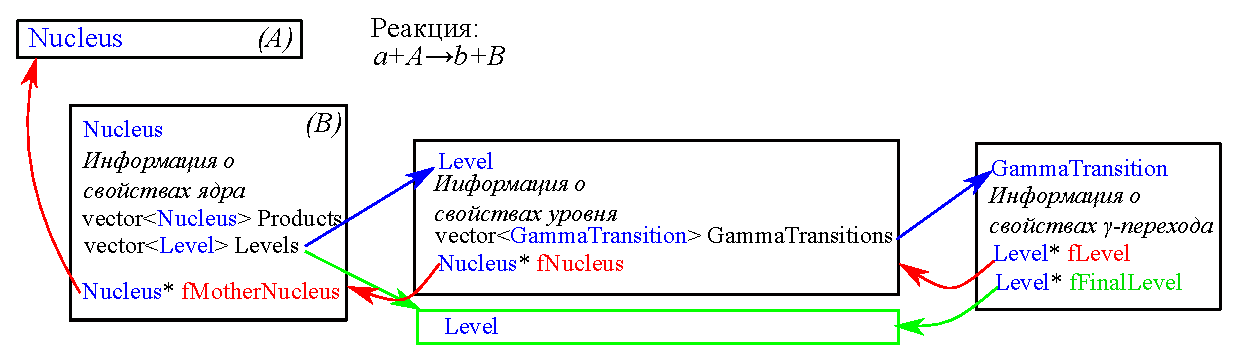
\includegraphics[width=1\linewidth]{TalysLibScheme.eps}}
\caption{Иерархия классов библиотеки TalysLib.}
\label{fig:TalysLibStructure}
\end{figure}
Для ввода и вывода информации TALYS использует текстовые файлы, более того, с их помощью осуществляется коммуникация между кодом ECIS, выполняющим все расчеты в рамках оптической модели и подхода связанных каналов, и остальной программой, в которой происходят расчеты компаунд-процессов. Входной файл TALYS имеет простую и легкую для заполнения форму, в то же время, структура файлов, хранящих информацию о деформациях и оптических потенциалах конкретных ядер, довольно сложная и требует ввода параметров в формате с фиксированной шириной и положением полей данных. Применение библиотеки TalysLib позволяет существенно упростить заполнение входных файлов TALYS и уменьшить количество возможных ошибок. Файловый ввод-вывод позволяет достаточно просто реализовать запуск TALYS с помощью системных вызовов.

Считывание результатов вычислений производится из выходного файла TALYS, что, во-первых, упрощает контроль за правильностью получаемых результатов, а, во-вторых, сокращает количество создаваемых после вычислений файлов, что увеличивает скорость работы. Кроме того, для ускорения вычислений файлы сохраняются на виртуальный диск в оперативной памяти, что исключает их запись на жесткий диск.\par
%\section{Применение TalysLib}
Изначально TalysLib создавалась для автоматизированной расшифровки и аппроксимации $\gamma$-спектров, получаемых при исследовании нейтрон-ядерных реакций. Обычно для решения этих задач используются данные из ENSDF, но у данного подхода есть недостатки, связанные, во-первых, с достаточно сложной структурой файлов ENSDF, а, во-вторых, с невозможностью оценки выходов $\gamma$-линий непосредственно из информации, представленной в ENSDF, что может привести к ошибкам в идентификации фотопиков. Использование же результатов расчетов в TALYS имеет следующие преимущества:
\begin{itemize}
\item Структура выходного файла TALYS значительно более проста, чем файла ENSDF,
\item В выходном файле TALYS записаны только возможные при данной энергии налетающего нейтрона $\gamma$-переходы,
\item Для каждого $\gamma$-перехода вычисляется сечение, что позволяет, провести их отбор по интенсивности и избежать ошибок в идентификации близких по энергии фотопиков,
\item Полученные на основе вычисленных сечений соотношения амплитуд близких $\gamma$-пиков могут быть использованы как начальные приближения при их аппроксимации.
\end{itemize}
Пример применения TalysLib для расшифровки $\gamma$-спектров показан на Рис. \ref{fig:SpectrumDecodingExample}.\par
\begin{figure}
\center{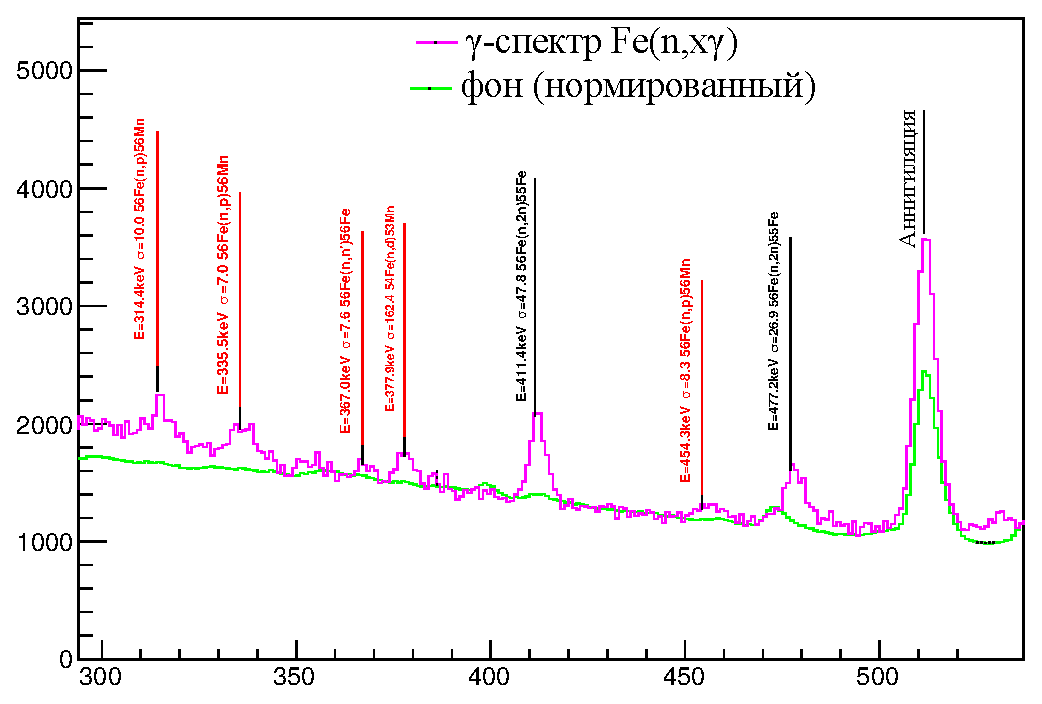
\includegraphics[width=1\linewidth]{TalysLibSpectrum.eps}}
\caption{Пример расшифровки спектра $\gamma$-лучей, полученного в эксперименте с железом, с помощью TalysLib. Красным выделены $\gamma$-переходы, ранее не наблюдавшиеся в реакциях ($n,x\gamma$).}
\label{fig:SpectrumDecodingExample}
\end{figure}
\begin{figure}
\center{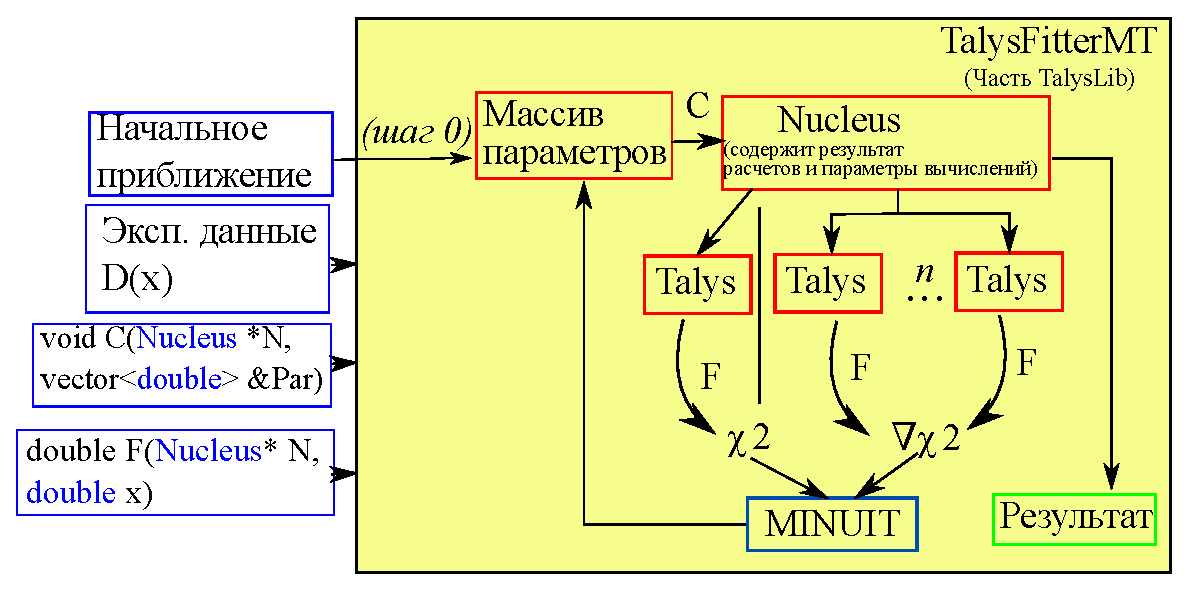
\includegraphics[width=0.8\linewidth]{MinimisationSketch.eps}}
\caption{Блок-схема процедуры минимизации.}
\label{fig:MinimizationProcedure}
\end{figure}
Другой областью применения TalysLib является подбор параметров моделей в TALYS для улучшения согласия результатов расчетов и экспериментальных данных. Для выполнения этой процедуры требуется проведение большого количества вычислений, которые необходимы для рассчета градиентов минимизируемой функции. Структура TalysLib позволяет выполнять подбор практически любого числового параметра модели к любому набору экспериментальных данных. Данный функционал реализован с помощью класса TalysFitterMT и минимизатора MINUIT, встроенного в ROOT. Для выполнения минимизации необходимы две задаваемые пользователем функции \textit{C} и \textit{F}, первая из которых сопоставляет набор подбираемых параметров с параметрами вычислений, а вторая описывает процедуру извлечения данных, соответствующих экспериментальным, из основных классов библиотеки. Блок-схема процедуры минимизации приведена на Рис. \ref{fig:MinimizationProcedure}.

Саму минимизирующую процедуру можно описать следующим образом: для начала процедуры необходим некоторый начальный набор параметров, который может быть взят непосредственно из параметров модели <<по-умолчанию>>, либо задан пользователем. Также нужна некоторая выборка экспериментальных данных, представимая в виде таблично заданной функции одной переменной \textit{D(x)}, например, дифференциальное сечение упругого и неупругого рассеяния на первом возбужденном состоянии может быть представлено как 
\begin{equation}
D(x)=
	\begin{cases}
	\frac{d\sigma^{el}}{d\Omega}(x), & x\leq 180;\\
	\frac{d\sigma^{inl}}{d\Omega}(x-180) & x>180.
	\end{cases}
\end{equation}
Аналогичным образом могут быть заданы функции $D^{err}_x(x)$ и $D^{err}_y(x)$, описывающие ошибки эксперимента.
Требуемые для сопоставления параметров модели и минимизируемых параметров, а также результатов расчета и экспериментальных данных функции \textit{C} и \textit{F} задаются пользователем, а указатели на них передаются в класс TalysFitterMT, где они используются для вычисления $\chi^2$ и $\mathbf{\nabla} \chi^2$:
\begin{equation}
\chi^2=\sum\limits_{i=0}^N\frac{((D(x_i)-F(x_i))^2}{(D^{err}_x(x_i))^2+(D^{err}_y(x_i))^2}
\end{equation}

Процедура подбора параметров начинается с расчета $\chi^2$ и $\mathbf{\nabla} \chi^2$ для начального приближения, которые затем передаются в MINUIT. На основе вычисленного $\mathbf{\nabla} \chi^2$ MINUIT определяет набор лежащих на градиенте точек, координаты которых с помощью функции $C$ передаются в объект Nucleus, который создает новые входные файлы для TALYS. С их помощью в этих точках снова рассчитывается $\chi^2$, и определяется набор параметров, для которого эта величина является наименьшей. Для него вычисляется $\mathbf{\nabla} \chi^2$ и цикл повторяется. После прохождения некоторого количества циклов MINUIT инициирует завершение процедуры минимизации. 

Расчеты в TALYS могут выполняться довольно продолжительное время, особенно, если используются отличные от DWBA подходы для описания прямых реакций. В случае задачи оптимизации $N$ параметров требуется для каждого расчета $\mathbf{\nabla} \chi^2$ требуется $2N$ запусков TALYS. К счастью, вычисление  $\mathbf{\nabla} \chi^2$ может быть легко выполнено в многопоточном режиме путем запуска нескольких копий TALYS одновременно, что ускоряет процедуру минимизации примерено в 6 раз для задачи с N=11. 

За ходом процесса минимизации можно наблюдать: текущий результат расчета и величины $\chi^2$ выводятся в реальном времени, как показано на Рис. \ref{fig:MinimizationPicture}.
 \begin{figure}
\center{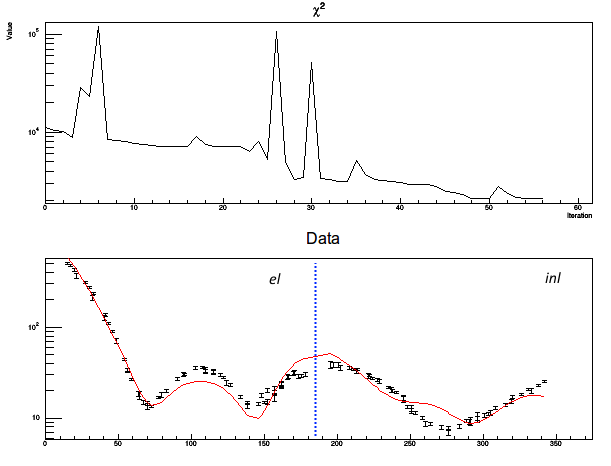
\includegraphics[width=1\linewidth]{Minimization.png}} 
\caption{Пример работы минимизирующей процедуры. Сверху~--~значения $\chi^2$, снизу~--~экспериментальные данные в виде $D(x)$ (точки), результаты расчета (линия). Данные, соответствующие упругому и неупругому рассеянию, разделены пунктирной линией.}
\label{fig:MinimizationPicture}
\end{figure}
Выбросы на графике $\chi^2$ (Рис.~\ref{fig:MinimizationPicture}.) связаны с расчетами в разных точках, лежащих на градиенте, необходимых для выбора набора параметров, который будет использоваться на следующем шаге минимизации. Видно, что величина $\chi^2$, в среднем, убывает с каждой итерацией.

\section{Структура библиотеки}
Библиотека состоит из набора классов, описывающих различные физические свойства ядер, <<классов управления>> и классов хранения данных. В данном разделе перечислены и описаны созданные для библиотеки пользовательские классы. 
\subsection{Класс TalysLibManager}
<<Управляющий>> класс
\subsection{Класс Nucleus}
Класс Nucleus включает в себя набор объектов и методов для работы со свойствами ядра. Описание методов и членов этого класса приведено ниже
\subsubsection{string Name,Reaction,Projectile}
Name -- строка string, содержащая имя ядра вида "56Fe".

Reaction -- строка string, содержащая реакцию, приводящая к образованию данного ядра, строка вида "(n,p)".

Projectile -- строка string, содержащая, налетающую частица, строка вида "n". Возможные значения данного параметра: n, p, d, t, h, a, g.
\subsubsection{vector<Level> Levels}
Вектор, содержащий объекты типа Level-информацию о свойствах ядерных уровней.
\subsubsection{OpticalModelParameters OMPN, OMPP}
Объекты, класса OpticalModelParameters, содержащие в себе информацию об оптическом потенциале для нейтронов (OMPN) и протонов (OMPP).
\subsubsection{Deformation Def}
Объект, класса Deformation, содержащий в себе сведения о деформации ядра в основном и возбужденных состояниях, а так же о природе этих состояний.
\subsubsection{TGraph ElacticTotTalys, ElasticDirectTalys, ElasticCompoundTalys}
Графики углового распределения упруго рассеянных частиц:  ElacticTotTalys -- полное сечение, ElasticDirectTalys -- прямая компонента упругого рассеяния, ElasticCompoundTalys -- компаунд-компонента. Данные графики заполняются функцией Nucleus::GetElasticAngularDistribution(string type, string option) из векторов Angle, ElTot; Angle, ElCompound; Angle, ElDirect соответственно.
\subsubsection{InelasticTotTalysV, InelasticDirectTalysV, InelasticCompoundTalysV, ElasticTotTalysV, ElasticDirectTalysV, ElasticCompoundTalysV, TotTalysV}
Графики сечений в зависимости от некоторого, определяемого пользователем, параметра V. Заполняются функцией Nucleus::AddPoint(double x_value, Nucleus* Nucl) из значений TotInelastic, CompoundInelastic, DirectInelastic, TotElastic, CompoundElastic, DirectElastic,  TotTalys соответственно. Величины TotInelastic, CompoundInelastic, DirectInelastic, TotElastic, CompoundElastic, DirectElastic,  TotTalys, в свою очередь, считываются непосредственно из output файла функцией Nucleus::ReadElastic().
\subsubsection{BNECS_gamma, BNECS_neutron, BNECS_proton, BNECS_deuteron, BNECS_triton, BNECS_3He, BNECS_alpha}
Данные графики представляют собой полные сечения рождения частиц $\gamma$, n, p, d, $^3$H, $^3$He, $\alpha$ соответственно, в выходном файле данные величины названы <<Binary non-elastic cross sections (non-exclusive)>>. Заполнение этих графиков производится функцией Nucleus::AddPoint(double x_value, Nucleus* Nucl) из величин BNECS_g, BNECS_n, BNECS_p, BNECS_d, BNECS_t, BNECS_tau, BNECS_a соответственно, а они, в свою очередь, считываются из output файла функцией Nucleus::ReadElastic().
\subsubsection{TEISGraphTot, TEISGraphCont, TEISGraphDiscr}
Данные графики представляют собой сечения неупругого рассеяния, т.е., реакций вида $(n,1nx)$: полное, в континууме и на дискретных уровнях соответственно, в выходном файле данные величины названы <<Total exclusive Inelastic scattering>>. Заполнение этих графиков производится функцией Nucleus::AddPoint(double x_value, Nucleus* Nucl) из величин TEISTot,TEISCont,TEISDiscr соответственно, а они, в свою очередь, считываются из output файла функцией Nucleus::ReadElastic().
\subsubsection{void ReadElastic()}
Функция, считывающая output файл и записывающая в переменные TOTGamProd, TOTNProd, TOTPProd, TOTDProd, TOTAProd полные сечения образования $\gamma$, n, p, d, $\alpha$ соответственно;  в TotElastic, CompoundElastic, DirectElastic записываются сечения упругого рассеяния и вклады отдельных компонент, а в TotInelastic, CompoundInelastic, DirectInelastic - сечения неупругого рассеяния. В переменную TotTalys записываются значения полного сечения.
\subsubsection{TGraph* GetElasticAngularDistribution(string type,string option)}
Данная функция строит угловое распределение рассеянных нейтронов и возвращает указатель на соответствующий график. Переменная type задает возможные варианты графика. Возможные значения: "Total" - полное сечение, "Compound" - компаунд-компонента, "Direct" - прямая компонента. Аргумент option принимает 2 значения: "" (по-умолчанию) и "new". В первом случае функция вернет уже построенный график, во втором-перестроит его.
\subsubsection{int WriteOMPOrUseKoningP, WriteOMPOrUseKoningN}
Данные переменные задают алгоритм работы с оптической моделью для протонов и нейтронов соответственно. Если значение переменной равно -1, то в расчете будет использован потенциал "по-умолчанию", либо заданный в input файле, если WriteOMPOrUseKoning=0, то будет использован потенциал, считанный из базы TALYS. Этот потенциал может быть изменен пользователем. Если в базе потенциала для данного ядра нет, будет использован потенциал "по-умолчанию". В случае, если если WriteOMPOrUseKoning=1, то будет использован потенциал из базы, а если его не окажется-то потенциал Кёнинга. Если WriteOMPOrUseKoning=2, то будет использован потенциал Кёнинга вне зависимости от наличия в базе потенциала для данного ядра.
\subsubsection{void MergeLevels(float tolerancy)}
Функция, используемая для слияния уровней, считанных из TALYS и NDS. Использование в дальнейшем не предполагается.
\subsubsection{SortingLevels()}
Функция, выполняющая сортировку вектора Levels по энергии уровня. 
\subsubsection{FindProductsByReaction(string reaction)}
Функция, выполняющая поиск продукта по соответствующей реакции и возвращающая указатель на найденный продукт. В случае, если продукт не найден, возвращает NULL.
\subsubsection{FindProductByName(string _Name)}
Функция, выполняющая поиск продукта по его имени и возвращающая указатель на найденный продукт. В случае, если продукт не найден, возвращает NULL.
\subsubsection{Nucleus* fMotherNucleus}
Указатель на начальное ядро, если рассматриваемое ядро является продуктом реакции и содержится в векторе Products. В случае, если рассматриваемое ядро является начальным ядром, он равен NULL. Устанавливается функцией AssignPointers().
\subsubsection{Nucleus()}
Конструктор по-умолчанию. Необходим для корректной работы динамических контейнеров.
\subsubsection{Nucleus(string Name,string Reaction="")}
Конструктор. Принимает как аргумент Name-название ядра, например, "56Fe",  и Reaction-реакцию, в которой данное ядро образовалось. В случае начального ядра этот аргумент остается, по умолчанию, пустым. В процессе создания ядра данным конструктором выполняются считывание из базы TALYS величин Z, A, распространенности изотопа, схемы уровней, параметорв деформации и оптических потенциалов, выполняется присваивание указателей на данное ядро для уровней, деформаций и оптических потенциалов.
\subsubsection{Nucleus(NucleusData ND)}
Конструктор, позволяющий создать объект Nucleus из более компактного объекта NucleusData. В силу технических ограничений, не удалось реализовать запись объекта Nucleus в .root файл, возможно, эта проблема связана с указателями. Объект NucleusData записывается в .root файл и считывается из него без каких-либо проблем.
\subsubsection{ReadENSDFFile(string filename="",string Nuclide="")}
Функция, считывающая ENSDF файлы и заполняющая уровни (Levels). Использование в дальнейшем не предполагается.
\subsubsection{ReadLevelsFromTalysDatabase(string type="final")}
Функция, считывающая параметры уровней из базы TALYS. В качестве аргумента принимает тип информации об уровнях. Возможные значения аргумента: "final", "exp", "hfb", описание приведено в TALYS manual (v 1.9), p. 137.
\subsubsection{SetProjectileEnergy(double E)}
Функция, устанавливающая энергию начальной частицы в МэВ.
\subsubsection{vector<Level*> GetLevelsWithCorrespondingTransitions(float Energy, float tolerancy=1, float intensity=0)}
Функция, выполняющая поиск уровней с гамма-переходами энергии Energy, энергия гамма-перехода может отличаться от заданной на tolerancy, интенсивность должна быть не ниже intensity. Использовалась для поиска подходящих гамма-переходов в данных, считанных из ENSDF (ну, или, NDS). Использование в дальнейшем не предполагается.
\subsubsection{Level* FindLevelFromTalys(float Energy, SpinParity JP)}
Функция, выполняющая поиск уровня, полученного из базы TALYS с данной энергией и спин-четностью JP. В случае успеха возвращает указатель на найденный уровень, в противном случае-NULL.
\subsubsection{Level* FindBestLevelByEJP(float Energy, SpinParity JP, float tolerancy=1)}
Функция, выполняющая поиск уровня, лучше всего подходящего под заданные энергии. В случае, когда есть несколько уровней в пределах tolerancy от Energy, лучшим будет признан тот, который имеет спин-четности, совпадающие с JP. В случае успеха возвращает указатель на найденный уровень, в противном случае-NULL.
\subsubsection{FindLevelByEnergy(float Energy, float tolerancy=1)}
Функция, выполняющая поиск уровня с энергией Energy, энергия уровня может отличаться на tolerancy от величины Energy. В случае успеха возвращает указатель на найденный уровень, в противном случае-NULL.
\subsubsection{Level* FindLevelByNumber(int number)}
Функция, выполняющая поиск уровня с данным порядковым номером (соответствует нумерации TALYS). Нумерация начинается с основного состояния, ему присвоен номер 0. В случае успеха возвращает указатель на найденный уровень, в противном случае-NULL.
\subsubsection{GammaTransition* GetBestTransition(float Energy, float tolerancy=1)}
Функция, выполняющая поиск гамма-перехода с энергией, наиболее близкой к Energy в пределах tolerancy. В случае успеха возвращает указатель на найденный уровень, в противном случае-NULL.
\subsubsection{vector<GammaTransition*> GetGammaTransition(float Energy, float tolerancy=1, float intensity=0)}
Функция, выполняющая поиск гамма-переходов с энергией, наиболее близкой к Energy в пределах tolerancy. Возвращает вектор указателей на найденные переходы.
\subsubsection{vector<GammaTransition*> GetGammaTransitions(string option="Talys",int BetterThan=100, float tolerancy=1, float intensity=0)}
Функция, выполняющая поиск гамма-переходов с происхождением и надежностью, задаваемыми аргументами функции. Использование в дальнейшем не предполагается.
\subsubsection{vector<Nucleus> Products}
Вектор, содержащий объекты типа Nucleus. В случае, когда рассматриваемое ядро является начальным, содержит ядра-продукты, в случае же, когдя рассматриваемое ядро само является продуктом, пуст. Заполняется функцией Nucleus::GenerateProducts().
\subsubsection{void GenerateProducts(string Projectile="n")}
Функция, выполняющая создание продуктов. Заполняет вектор Products, вызывает функции, выполняющие создание input файла для TALYS, его запуск и считывание результатов вычислений. В качестве аргумента принимает название начальной частицы.
\subsubsection{void ExecuteCalculationInTalys(string _Projectile="n")}
Функция, выполняющая создание входного файла для TALYS и запуск вычислений. В качестве аргумента принимает название начальной частицы. Во входной файл могут быть добавлены дополнительные команды, находящиеся в Nucleus::TalysOptions.
\subsubsection{void ReadTalysCalculationResult()}
Функция, выполняющая считывание результатов расчета TALYS. Считываются:
\begin{enumerate}
\item ADTot, ADDirect, ADCompound-угловые распределения неупруго рассеянных частиц и продуктов реакции и вклады прямых и компаунд-процессов
\item сечения излучения гамма-квантов
\end{enumerate} 
В теле данной функции выполняется приписывание гамма-переходов соответствующим уровням.
\subsubsection{void AssignSimilarLevels(float Tolerancy=1.5)}
Функция, выполняющая приписывание уровням близких по энергии. Была введена, чтобы перерабатывать огромное множество одинаковых уровней из ENSDF. Использование в дальнейшем не предполагается.
\subsubsection{void DrawLevelScheme(double MinTalysCS=0)}
Функция, отрисовывающая схему уровней на текущий \href{https://root.cern.ch/doc/master/classTCanvas.html}{Canvas}. В качестве аргумента принимает сечение излучения гамма-кванта, переходы с сечением менее MinTalysCS отрисованы не будут.
\subsubsection{void AssignPointers()}
Функция, приписывающая указателям правильные значения. Присваивает fMotherNucleus указатель на начальное ядро, Level->fNucleus-указатель на ядро, к которому относится данный уровень. Необходимо вызывать при копировании и после окончания записи в контейнер.
\subsubsection{void ErasePointers()}
Функция, вызывающая стирание указателей.
\subsubsection{void AssignDeformationsToLevels()}
Функция, приписывающая уровням указатель на соответствующий объект LevelDeformation, содержащий информацию о деформации уровня и его происхождении. Приписывание деформаций осуществляется по номеру уровня.
\subsubsection{void SetLevelDeformation(int LevelNumber,char LevT, int BandN=-1, int BandL=-1, int NPhon=-1, int MagN=-1, vector<float> *Def=0)}
Функция, позволяющая установить деформацию для уровня c номером LevelNumber. В случае, если аргумент = -1, он будет пропущен при записи деформации в файл. Параметры деформации описаны в TALYS manual (v 1.9), p. 138, LevT соответствует типу уровня (type of collectivity), BandN-номер полосы (the number of band), BandL-момент полосы или мультипольность(?) (multipolarity), NPhon-число фононов (phonon number of the level), MagN-магнитное квантовое число (magnetic quantum number). Значения деформации ($\beta_2...\beta_8$) передаются с помощью указателя на вектор *Def.
\subsubsection{void SetLevelDeformation(double LevelEnergy,char LevT, int BandN=-1, int BandL=-1, int NPhon=-1, int MagN=-1, vector<float> *Def=0)}
Функция, позволяющая установить деформацию для уровня c энергией LevelEnergy (точность задания энергии должна быть лучще 1 кэВ). В случае, если аргумент = -1, он будет пропущен при записи деформации в файл. Параметры деформации описаны в TALYS manual (v 1.9), p. 138, LevT соответствует типу уровня (type of collectivity), BandN-номер полосы (the number of band), BandL-момент полосы или мультипольность(?) (multipolarity), NPhon-число фононов (phonon number of the level), MagN-магнитное квантовое число (magnetic quantum number). Значения деформации ($\beta_2...\beta_8$) передаются с помощью указателя на вектор *Def.
\subsubsection{string PrintLevels()}
Функция, возвращающая список уровней данного ядра в виде строки.
\subsubsection{string PrintReactions()}
Функция, возвращающая список продуктов и реакций, если данное ядро является начальным.
\subsubsection{string ReactionToTalysNotation(char DataSelection=kExcitationCS)}
Функция, генерирующая ключевое слово, по которому сведения о реакции, которая привела к рождению данного ядра, можно найти в файле. В качестве аргумента принимает тип информации, для которого должно быть сгенерировано ключевое слово. Возможные значения аргумента: kExcitationCS-сечение образования конкретного состояния, kAngularDistribution-угловое распределение частицы-продукта, kTotalInelasticCS-полное сечение образования данного продукта.
\subsubsection{float GetMass()}
Функция, возвращающая массу ядра в МэВ.
\subsubsection{NucleusData ToNucleusData()}
Функция, конвертирующая объект Nucleus в NucleusData, который может быть сохранен в .root файл.
\subsubsection{void GenerateGammaSpectrum(TH1F *Spectrum, TF1* ResolutionFunction, int NEntries=100000)}
Функция, позволяющая сгенерировать ожидаемый гамма-спектр на основе результатов вычислений в TALYS. Первый аргумент-указатель на гистограмму, куда будет записан спектр, второй-указатель на функцию \href{https://root.cern.ch/doc/master/classTF1.html}{(TF1)}, описывающую разрешение детектора, третий-число событий в спектре.
\subsubsection{void SetTGraphNameAndTitle(string ValName)}
Функция, задающая имена и подписи осей для графиков. В качестве аргумента принимает имя переменной, которая соответствует оси $x$.
\subsubsection{void AddPoint(double x_value, Nucleus* Nucl)}
Функция, выполняющая заполнение графиков InelasticTotTalysV, InelasticDirectTalysV, InelasticCompoundTalysV, ElasticTotTalysV, ElasticDirectTalysV, ElasticCompoundTalysV, TotTalysV, BNECS_gamma, BNECS_neutron, BNECS_proton, BNECS_deuteron, BNECS_triton, BNECS_3He, BNECS_alpha, TEISGraphTot, TEISGraphCont, TEISGraphDiscr значениями, находящимися в объекте, на который указывает указатель Nucleus* Nucl, в качестве переменной $x$ передается x_value. Вызывает аналогичную функцию для уровней (void Level::AddPoint(double x_value,Level *level)). Используется классом TalysCalculation для построения графиков зависимости результатов вычислений от переменных, задаваемых пользователем.

\subsection{Класс TalysCalculation}
Класс TalysCalculation включает в себя набор объектов и методов для работы с вычислениями в TALYS. Присутствуют методы для запуска расчётов, изменения параметров вычислений. Описание методов и членов этого класса приведено ниже
\subsubsection{Results, FinalResult}
В FinalResult хранится расчёт с максимальным значением параметра, в нем будут графики для неупругих сечений
\subsubsection{Target, Proj}

\subsubsection{TalysOptions}

\subsubsection{Variable}

\subsubsection{Elastic, Inelastic, GeneratedGraphs}

\subsubsection{VarValues}
Вектор значений параметров деформации, которые перебираются при вариации. Можно задать с помощью функции TalysCalculation::SetVarValues(min,max,step).
\subsubsection{GeneratedGraphs}

\subsubsection{ProjectileEnergy}

\subsubsection{void ReadParametersFromFile(string filename)}
Функция, 
\subsubsection{void ExecuteCalculation(), void ExecuteCalculation(void (*VarChangeFunction)(Nucleus *Nuclide, double value))}
Функции, 
\subsubsection{void SetTarget(string _Target), void SetProjectile(string _Proj), void SetVarValues(double min, double max, double step)}
Функции, 
\subsubsection{void ExecuteCalculation(), ExecuteCalculation(void (*VarChangeFunction)(Nucleus *Nuclide,double value))}
Функции, 
\subsubsection{void GenerateGraphs()}
Функция, 
\subsubsection{TGraph* GetLevelExcitationCrossSection(double LevelEnergy, string NucleusName, string Option)}
Функция, 
\subsubsection{TGraph* GetGammaTransitionCrossSction(double GammaEnergy, string NucleusName)}
Функция, 
\subsubsection{TMultiGraph* GetAngularDistributionsForLevel(double LevelEnergy,string NucleusName, string type, string option, TLegend *leg)}
Функция, 
\subsubsection{TMultiGraph* GetElasticAngularDistributions(string type, string option, TLegend *leg)}
GetElasticAngularDistributions возвращает TMultiGraph с угловыми распределениями, соответствующими значениям VarValues.
\subsection{Класс OMPStorageData}
Класс для хранения данных (выполняет роль структуры). Наследник класса \href{https://root.cern/doc/master/classTObject.html}{TObject} программы \href{https://root.cern}{CERN ROOT}, гарантированно может быть записан в root-файл. 
\subsection{Класс OMPStorage}
Наследник класса OMPStorageData. Владеет своими гетерами и сеттерами для оптических параметров.
\subsubsection{OMPStorageData ToOMPStorageData()}

\subsection{Класс OpticalModelParametersData}
Наследник класса \href{https://root.cern/doc/master/classTObject.html}{TObject} программы \href{https://root.cern}{CERN ROOT}. Содержит в себе объекты класса OMPStorageData.
\subsubsection{OMPStorageData PotentialData, PotentialDispData, PotentialKoningData}
Объекты класса OMPStorageData, хранящие в себе наборы параметров для разных типов оптического потенциала:\\
PotentialData -- текущий (рабочий) набор.\\
PotentialDispData -- набор оптической дисперсионной модели.\\
PotentialKoningData -- набор для глобальной параметризации Кёнинга.
\subsection{Класс OpticalModelParameters}
Основной класс для работы с оптическими параметрами. Наследник класса OpticalModelParametersData. Содержит в себе данные и методы работы с оптическими параметрами ядра. Владеет своими гетерами и сеттерами для оптических параметров, которые используют гетеры и сеттеры класса OMPStorage.
\subsubsection{OpticalModelParametersData ToOpticalModelParametersData()}
Объект класса OpticalModelParametersData
\subsubsection{OMPStorage Potential, PotentialDisp, PotentialKoning}
Объекты класса OMPStorage
\subsection{Класс TalysFitter}
Класс TalysFitter нужен для подбора параметров оптического потенциала, лучше всего описывающие экспериментальные сечения. 
\subsubsection{bool Calculated}
=false;
\subsubsection{bool ParTrackingFlag}
=false;
\subsubsection{bool ParChanged}
=false;
\subsubsection{double x_val}

\subsubsection{TalysFitter(string NuclName)}
Конструктор класса
\subsubsection{Nucleus Nuclide}

\subsubsection{void (*ParAssignmentFunction)(TalysFitter *PointetToTF)}
\subsubsection{vector<double> PreviousParameters}
\subsubsection{vector<double> Parameters}
\subsubsection{vector<string> ParNames}
\subsubsection{TF1}
\subsubsection{TF1}
\subsubsection{void EnableParTracking()}
\subsubsection{void DisableParTracking()}
\subsubsection{void TrackParChanges()}
\subsubsection{double Eval(double *x, double *p)}
\subsubsection{double (*GetEvaluationResult)(double x_value,TalysFitter *PointetToTF)}
\subsubsection{TF1 GenerateTF1(string name, double x_min,double x_max)}

\subsection{Класс TalysFitterMT}
Класс TalysFitterMT нужен для многопоточного подбора параметров оптического потенциала, лучше всего описывающие экспериментальные сечения. 

\end{document}
